\documentclass{article}

% Margins.
\setlength{\oddsidemargin}{0in}
\setlength{\evensidemargin}{0in}
\setlength{\headheight}{12pt}
\setlength{\headsep}{42pt}
\setlength{\topmargin}{-54pt}
\setlength{\textwidth}{6.5in}
\setlength{\textheight}{9in}

\usepackage{float}
\usepackage{graphicx}
% Drawing.
\usepackage{pgf}
\usepackage{tikz}

% Listings for formatting code.
\usepackage{listings}
% General options.
\lstset{breaklines=true, basicstyle=\small\ttfamily, tabsize=4, numbers=left, stepnumber=1, frame=single, showstringspaces=false}
% C++ specific high-lighting. Comments are 50/50 shades of green/black and strings coloured with 60/40 red/black mixture.
\lstset{language=[ISO]C++, commentstyle=\color{green!50!black}, keywordstyle=\color{blue}, stringstyle=\color{red!60!black}}

%opening
\title{Programming for Engineers I\\Lab 08\\Arrays}
\author{Hina Ashraf\and Attique Dawood}

\begin{document}
\maketitle
\section{What are arrays?}
Array is a special data-type. If we have a collection of data of same type as in the case of storage of ages of 100 students, arrays can be used. Arrays are data structure in which identical data types are stored.
\section{Declaration}
\begin{lstlisting}[caption={Array declaration}]
datatype ArrayName[Size]; // Size must be constant.
Example: int myArray[10];
         float AnotherArray[33];
         char aString[12];
\end{lstlisting}
\section{Initialization}
Array can either be initialised at declaration or at a later stage using loop.
\subsection{Initialisation at Declaration}
\begin{lstlisting}[caption={Array initialisation at declaration}]
int myArray1[10] = {0}; // Initialises whole array with zeroes.
int myArray2[10] = {-1,11,-12,10,15,2,4,-7,4,21}; // Initialise individual elements.
\end{lstlisting}
\subsection{Using \texttt{for} loop}
\begin{lstlisting}[caption={Array initialisation using for loop}]
int myArray1[10]; // Declaration.
for(int i=0; i<10; i++)
{
    myArray[i] = 0; // Initialise all elements to zero.
}
\end{lstlisting}
\section{Sample Program}
\begin{lstlisting}[caption={Sample program}]
#include <stdio.h>
int main()
{
    int Age[4]; // Declaration.
    Age[0] = 20;
    Age[1] = 19;
    Age[2] = 22;
    Age[3] = 21;

    printf{"First element  = %d\n", Age[0]);
    printf{"Second element = %d\n", Age[1]);
    printf{"Third element  = %d\n", Age[2]);
    printf{"Fourth element = %d\n", Age[3]);

    return 0;
}
\end{lstlisting}
\section{Copying Arrays}
Arrays cannot be copied using assignment operator, so individual elements must be copied using a loop. Similarly, other operations like addition, subtraction etc. must performed on individual elements rather than whole arrays.
\begin{lstlisting}[caption={Copying an array}]
#include <stdio.h>
int main()
{
    float Array1[5] = {-0.33f,-0.45f,0.22f,0.532f,0.101f};
    float Array2[5];

    // Copying...
    for (int i=0; i<5; i++)
    {
        Array2[i] = Array1[i];
    }
    // Display.
    for (int i=0; i<5; i++)
    {
        printf("Element %d = %f\n", i+1, Array2[i]);
    }

    return 0;
}
\end{lstlisting}

\section{Exercise}
\textbf{Question No. 1:} Declare a float array of size 10. Using loop take input from user. Calculate the sum and average of entire array. Print sum and average. And then print the array in reverse order.\\
\textbf{Question No. 2:} Declare an integer array of size 10. Using for loop take input from user. Take square of each integer and store it in the respective index. Print the array. Do all work in a single array.
\begin{figure}[H]
\centering
% \fbox{} can be removed. It only draws an outline around figure. Useful for trimming figure edges.
% Order of trimming is: trim= left bottom right top
\fbox{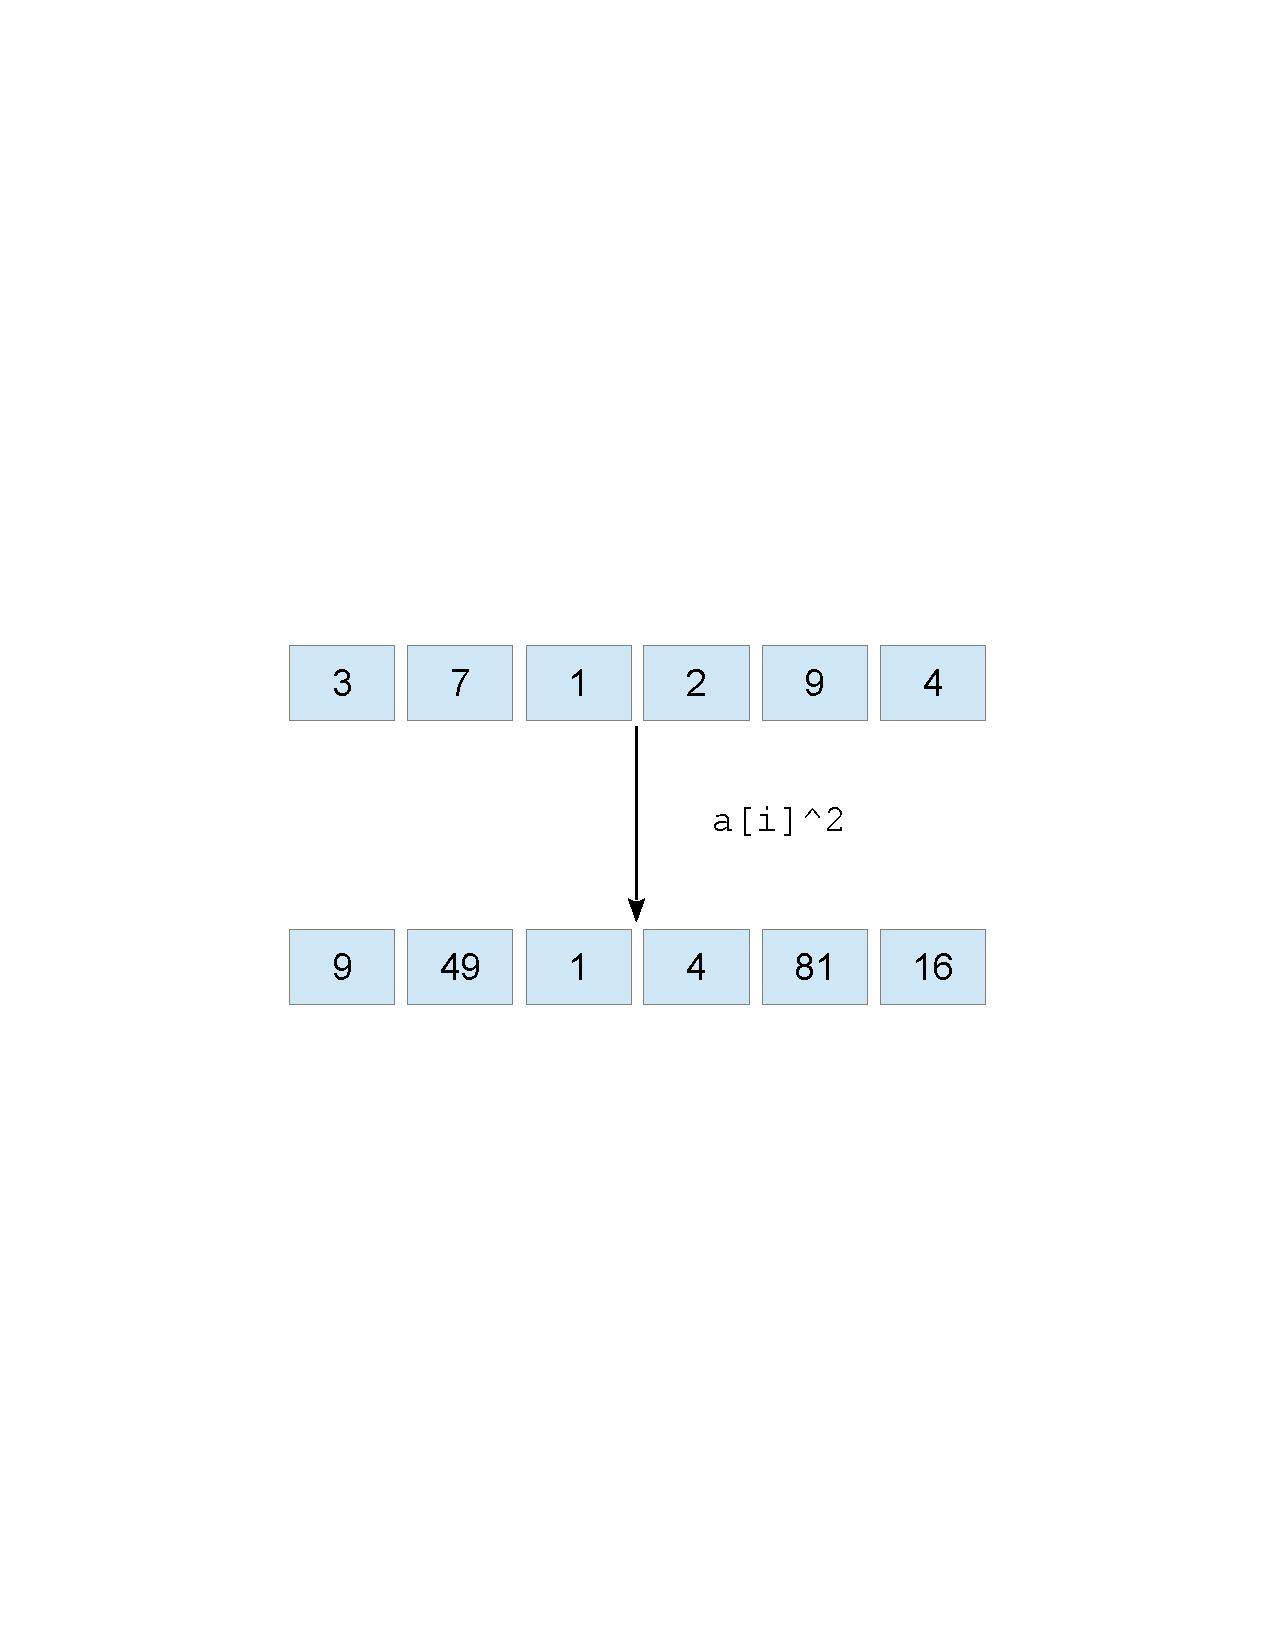
\includegraphics[scale=0.55, trim=4.5cm 10.5cm 4.5cm 10.5cm, clip]{ArraySquared.pdf}}
\caption{Squaring an array}
\label{Array-Squaring}
%\begin{tikzpicture}
%	% Writing 'original array'
%	\draw (-1.5cm,0.3cm) node {\textsf{Original Array:}};
%	% Drawing boxes.
%	\foreach \x in {0.0cm, 1.0cm, 2.0cm, 3.0cm, 4.0cm, 5.0cm, 6.0cm, 7.0cm}
%		\draw[thick] (\x, 0cm) rectangle (\x+1.0cm, 0.6cm);
%	% Writing numbers in boxes. This is original array.
%	\foreach \x/\y in {0.0cm/2, 1.0cm/3, 2.0cm/1, 3.0cm/8, 4.0cm/9, 5.0cm/10, 6.0cm/4, 7.0cm/6}
%		\draw (\x+0.5cm,0.3cm) node {\texttt{\y}};
%
%	% Drawing an arrow.
%	\draw[thick, ->, >=stealth] (4.0cm, -0.1cm) -- (4.0cm, -0.9cm);
%	
%	% Writing 'modified array'
%	\draw (-1.5cm,-1.3cm) node {\textsf{Squared Array:}};
%	% Drawing boxes.
%	\foreach \x in {0.0cm, 1.0cm, 2.0cm, 3.0cm, 4.0cm, 5.0cm, 6.0cm, 7.0cm}
%		\draw[thick] (\x, -1cm) rectangle (\x+1.0cm, -1.6cm);
%	% Writing numbers in boxes. This is modified array with \y storing squared values.
%	\foreach \x/\y in {0.0cm/4, 1.0cm/9, 2.0cm/1, 3.0cm/64, 4.0cm/81, 5.0cm/100, 6.0cm/16, 7.0cm/36}
%		\draw (\x+0.5cm,-1.3cm) node {\texttt{\y}};
%\end{tikzpicture}
\end{figure}
\textbf{Question No. 3:} Take an array of size 10. Initialize the array with 3's table using for loop. Now ask the user which integer you want to check in the array. If integer is present then print ``Yes integer is present its index no is [?]''\\
\end{document}
